\chapter{遅延聴覚フィードバックが身体運動に与える影響の調査の資料}
% 付録を掲載する場合,\verb|\chapter|コマンドの前に\verb|\appendix|コマンドを入れてください.
遅延聴覚フィードバックが身体運動に与える影響の調査を行うときに用いた,
研究参加同意書(明治大学生用・明治大学生以外の60歳未満の方用・明治大学生以外の60歳以上の方用),実験概要説明ボード(60歳の未満の方用・60歳以上の方用),聴力検査手順説明ボード,実験手順説明ボード,音量調整ボードを掲載する.
\begin{figure}[ht]
	\centering
	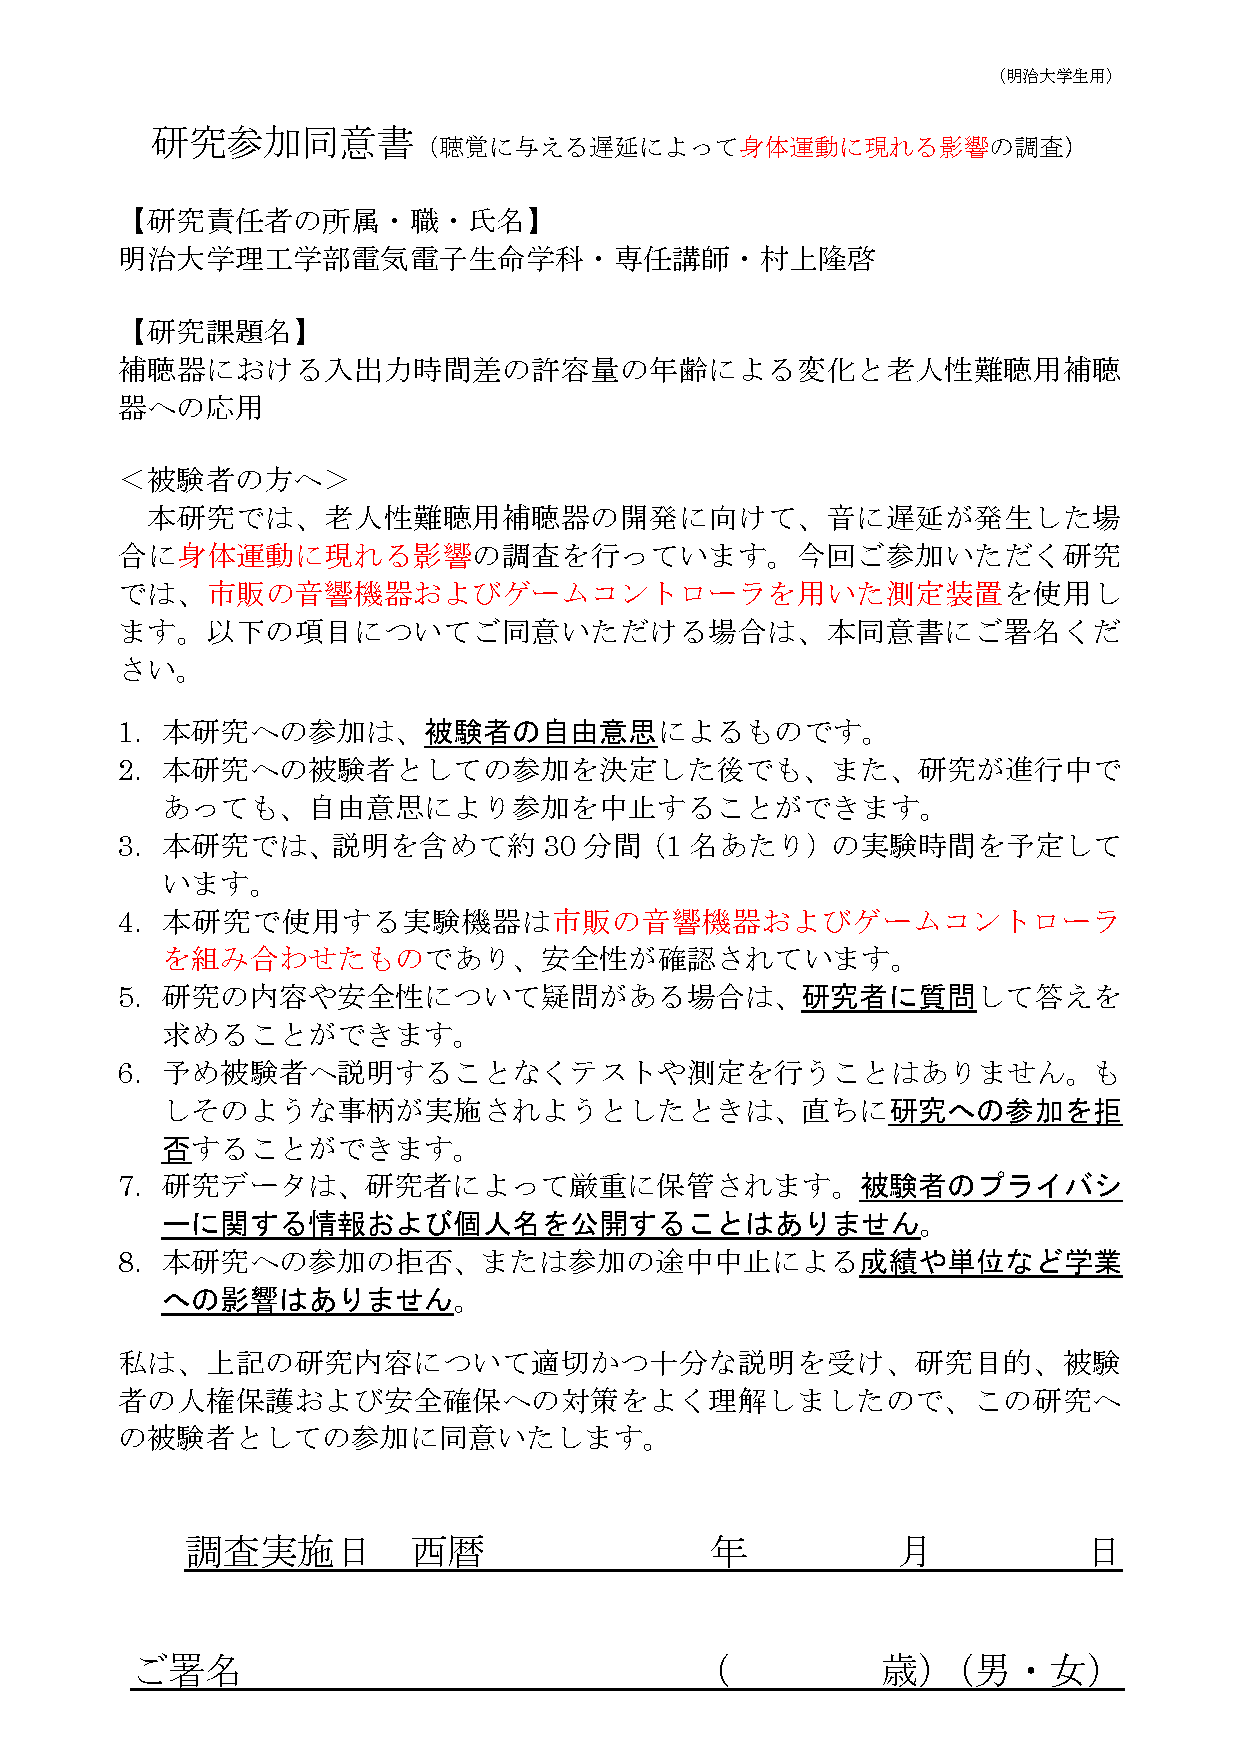
\includegraphics[width=\textwidth]{furoku_A/douisyo_meiji.pdf} % 画像の幅をテキストの幅に合わせる
	\caption{研究参加同意書(明治大学生用)}
\end{figure}
\begin{figure}[ht]
  \centering
  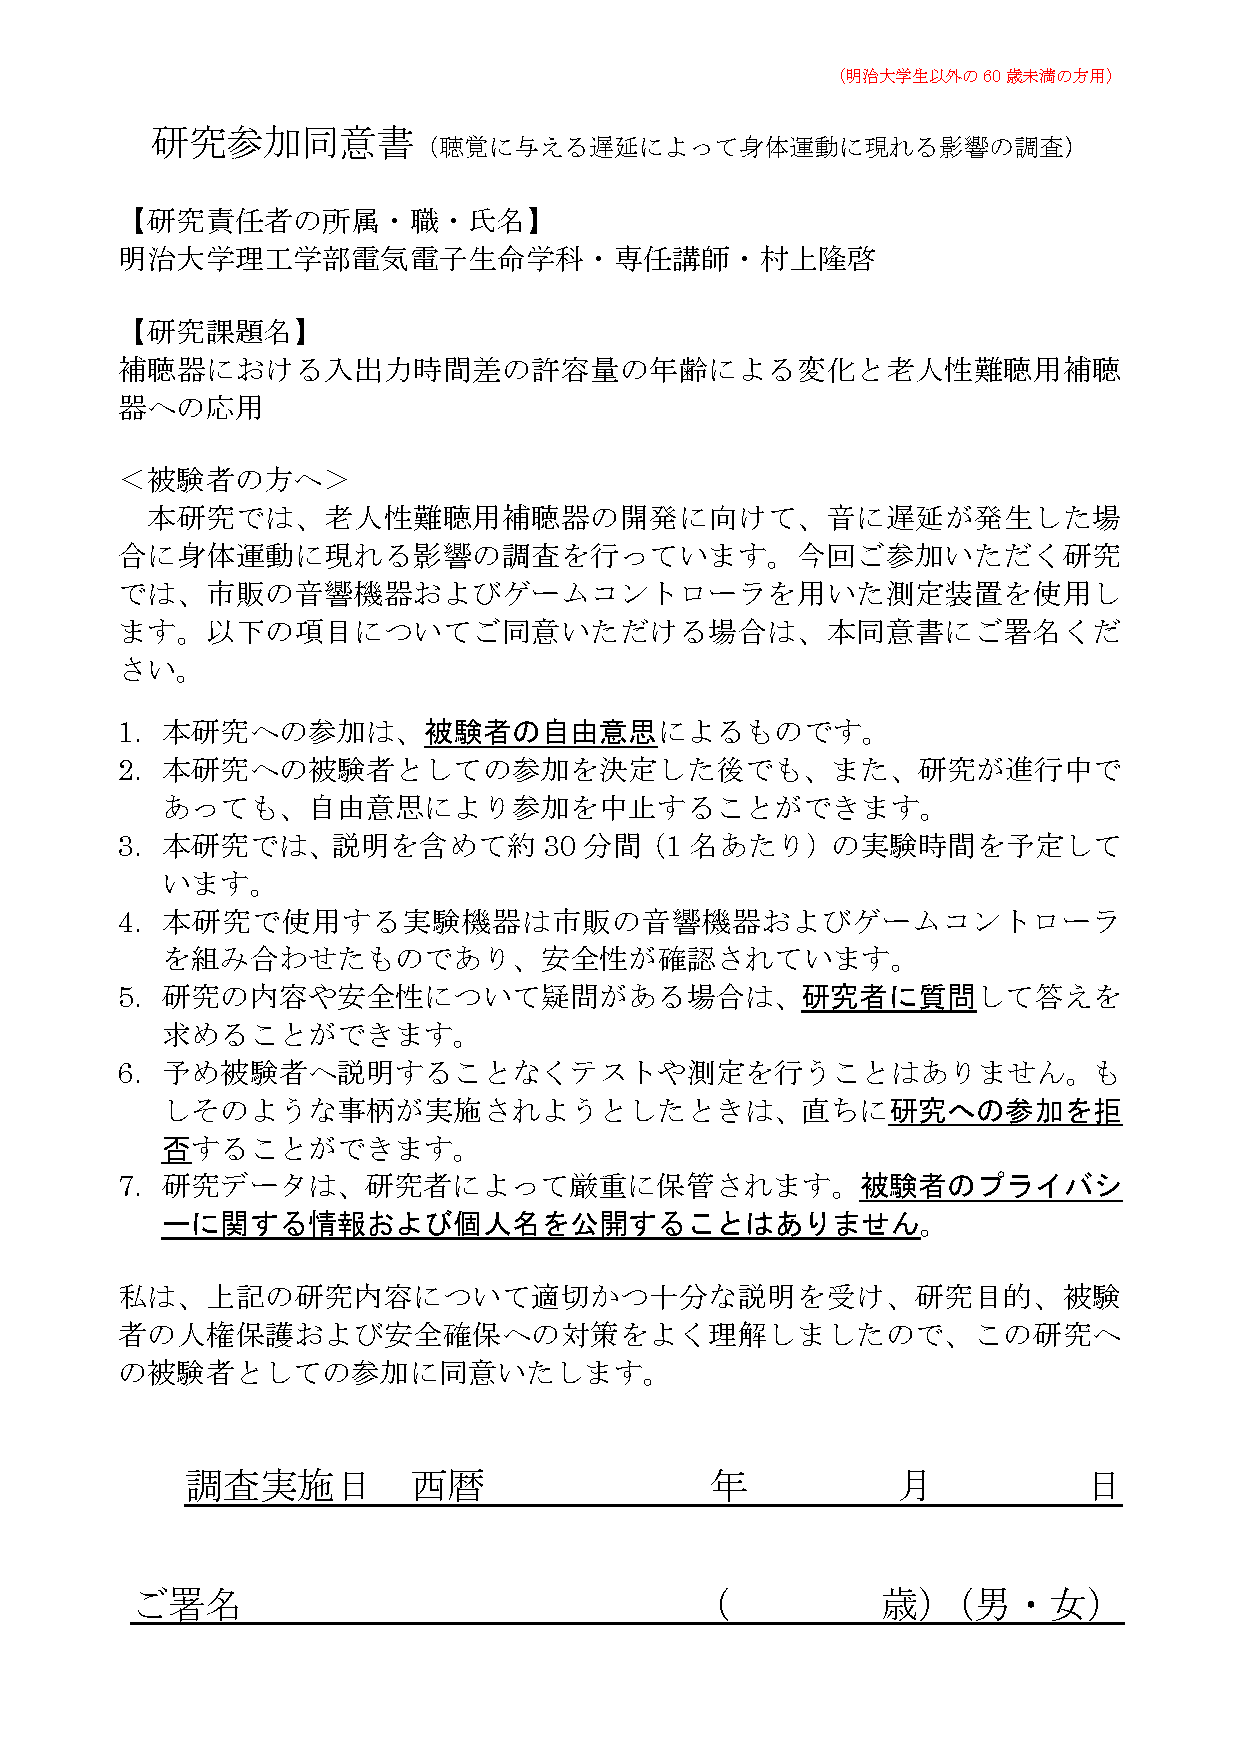
\includegraphics[scale=0.55]{furoku_A/Douisyo_Not60NotMeiji.pdf}
  \caption{研究参加同意書(明治大学生以外の60歳未満の方用)}
\end{figure}
\begin{figure}[ht]
  \centering
  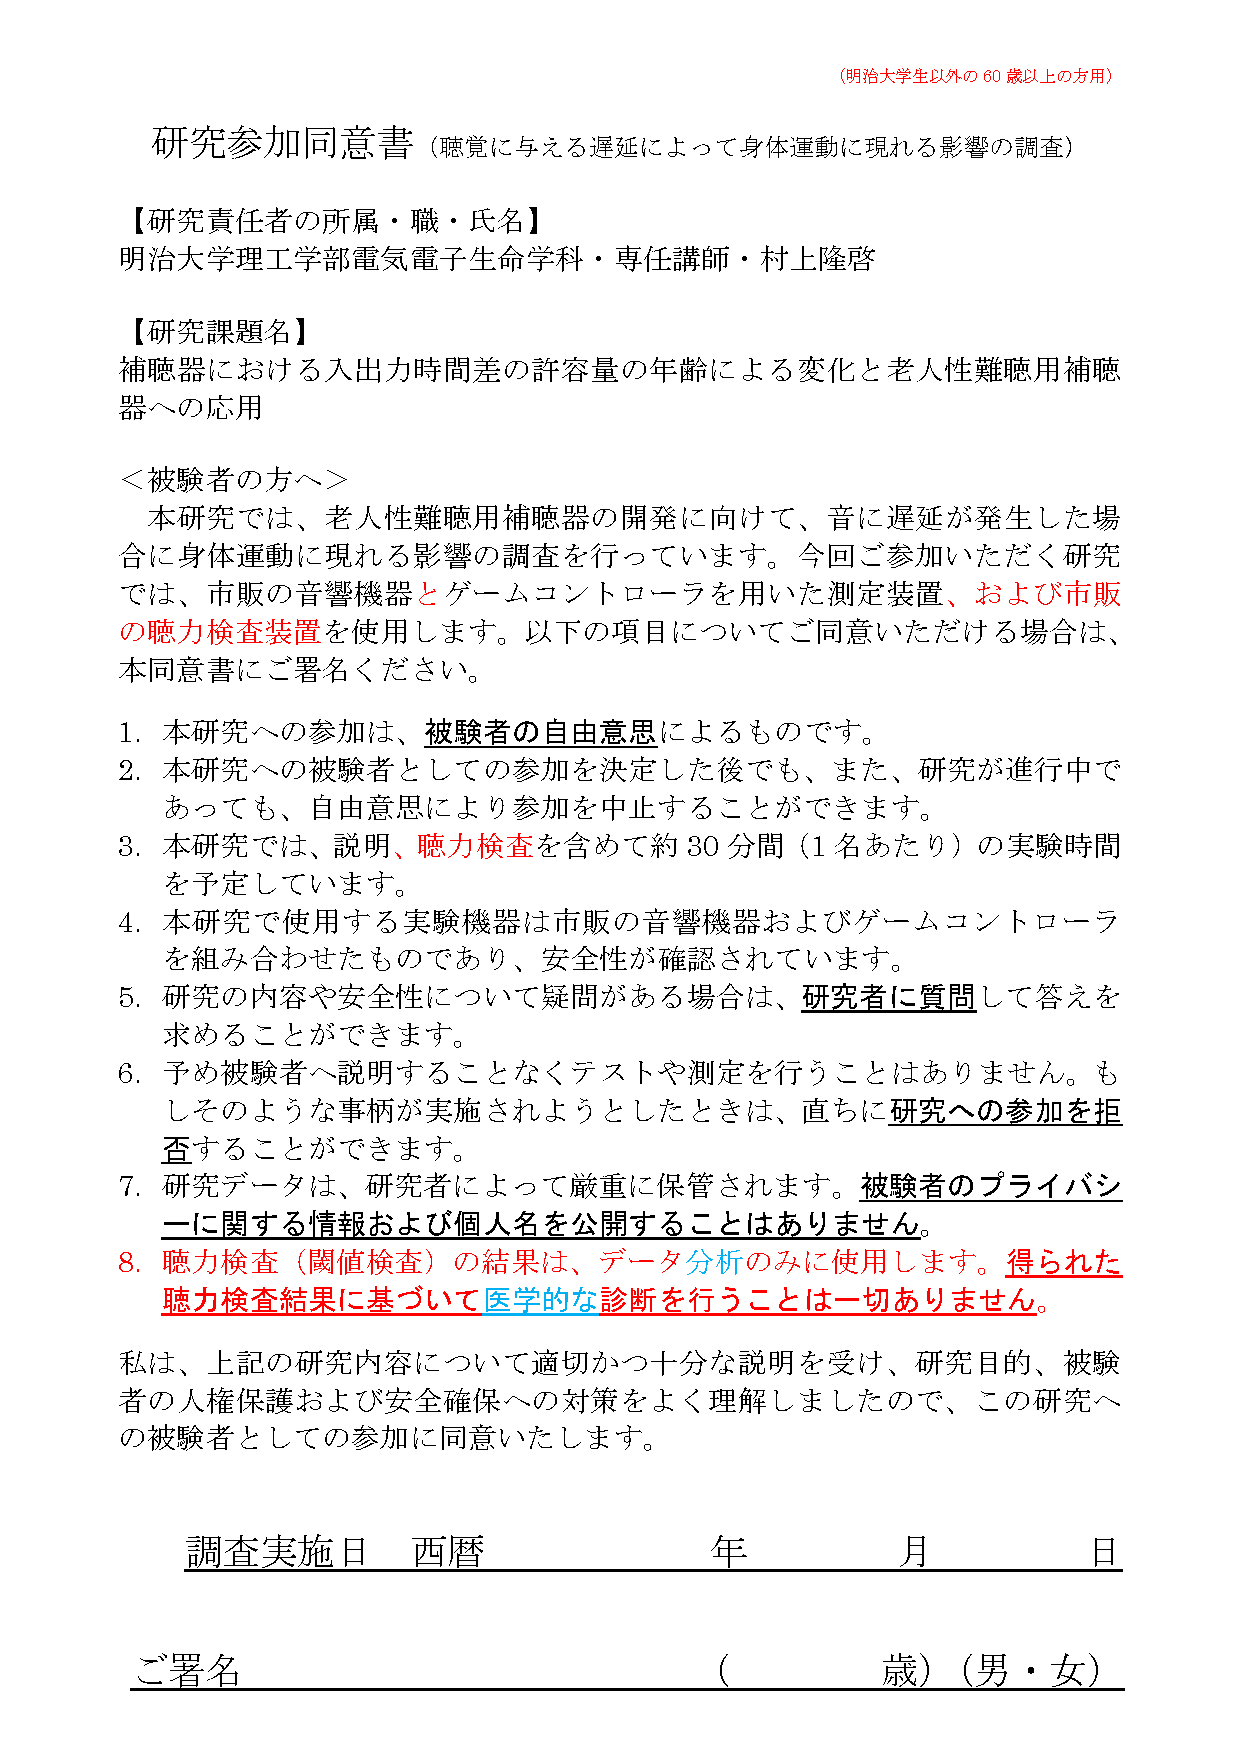
\includegraphics[scale=0.55]{furoku_A/Douisyo_60NotMeiji.pdf}
  \caption{研究参加同意書(明治大学生以外の60歳以上の方用)}
\end{figure}
\begin{figure}[ht]
  \centering
  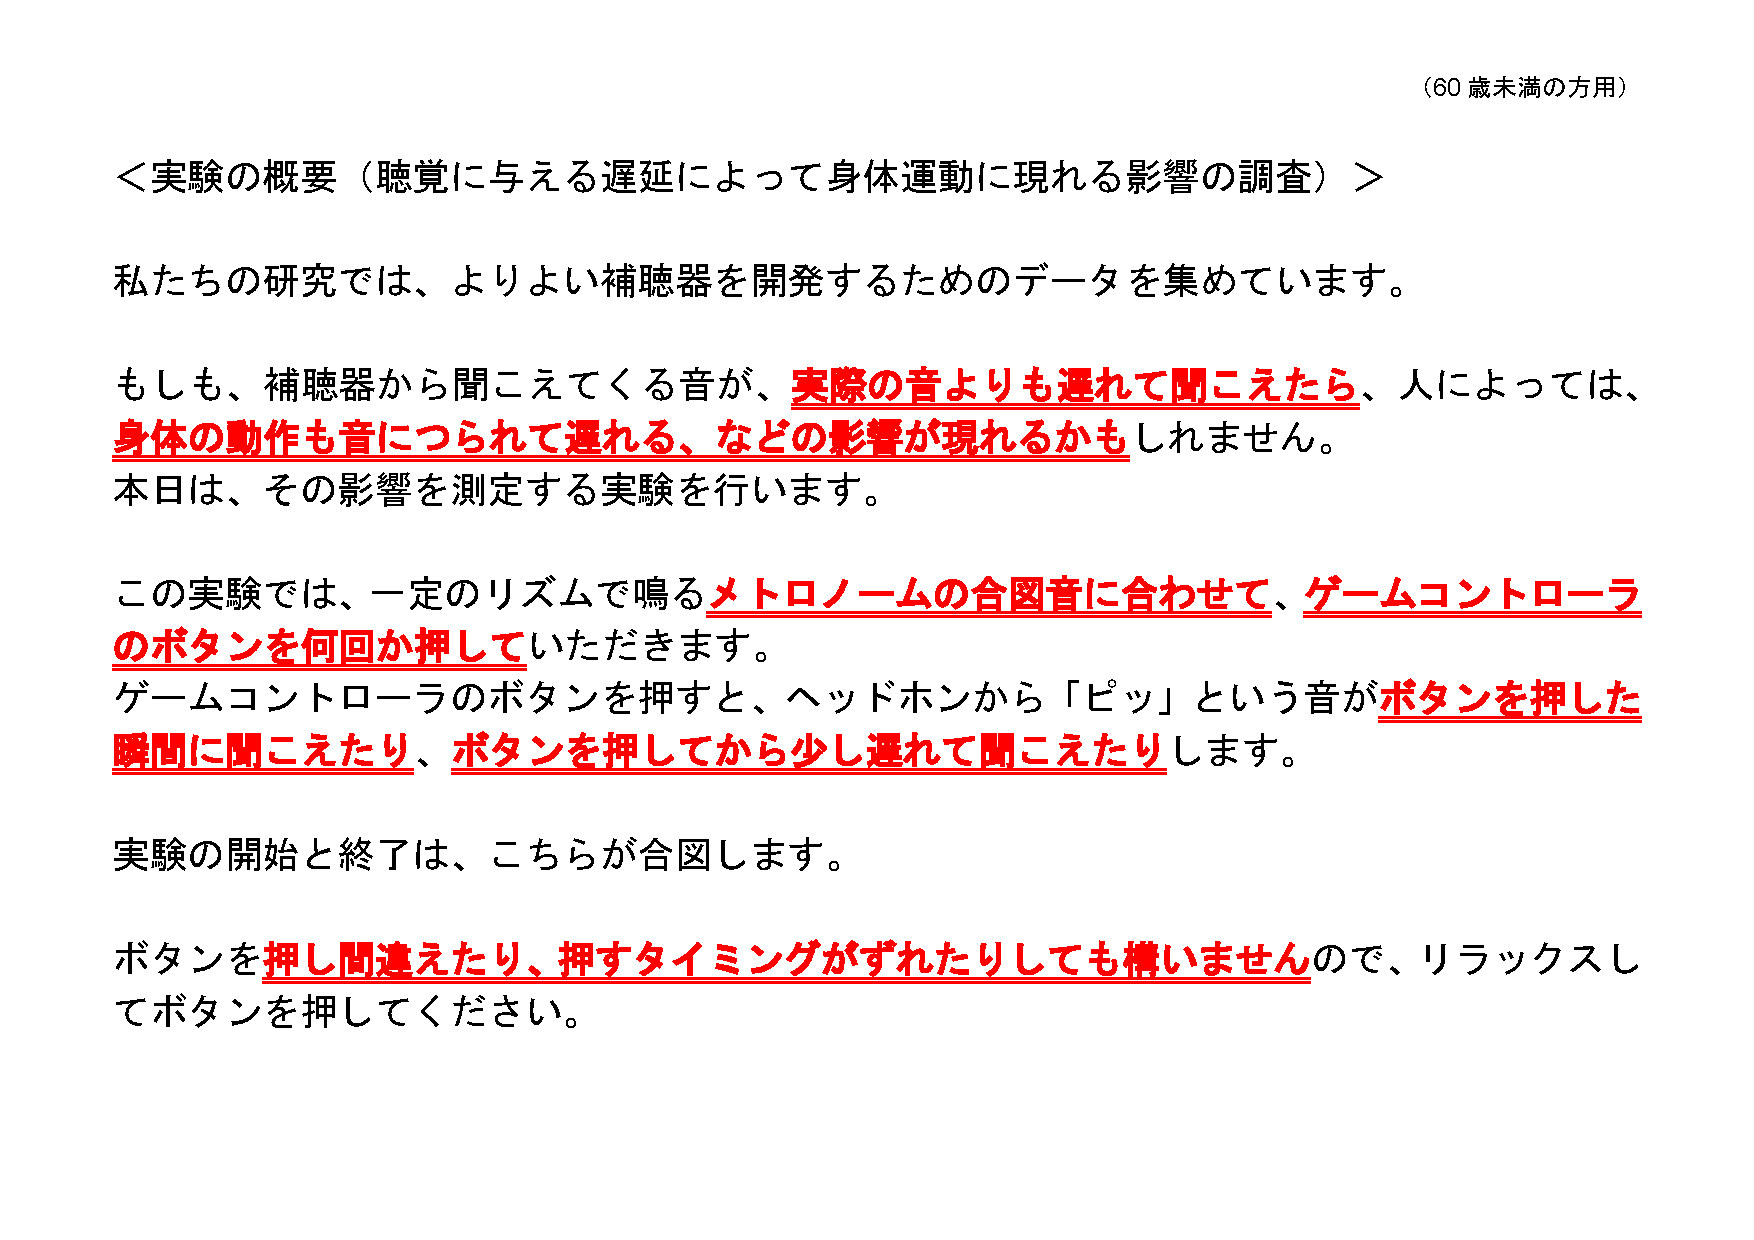
\includegraphics[scale=0.4]{furoku_A/Less60_gaiyou.pdf}
  \caption{実験概要説明ボード(60歳未満の方用)}
\end{figure}
\begin{figure}[ht]
  \centering
  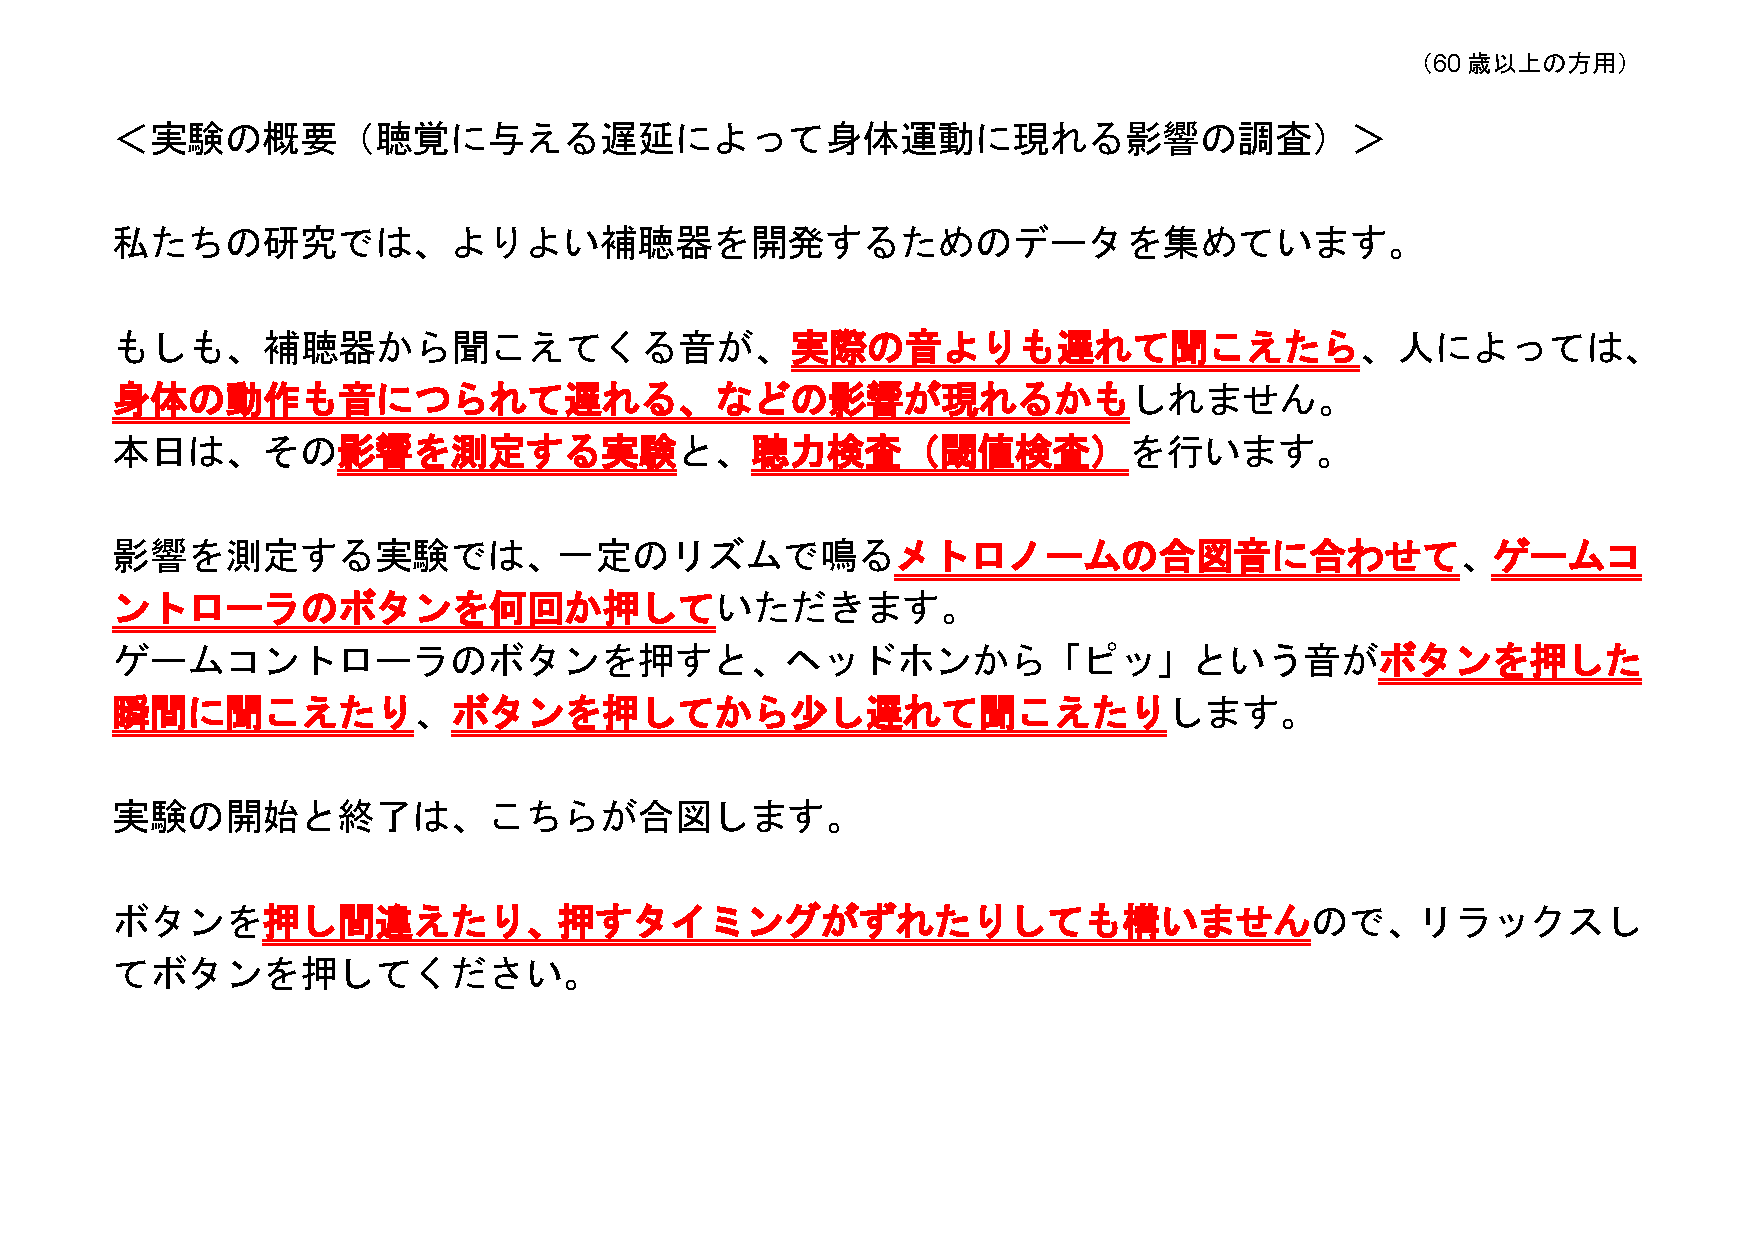
\includegraphics[scale=0.4]{furoku_A/MoreThan60_Gaiyou.pdf}
  \caption{実験概要説明ボード(60歳以上の方用)}
\end{figure}
\begin{figure}[ht]
  \centering
  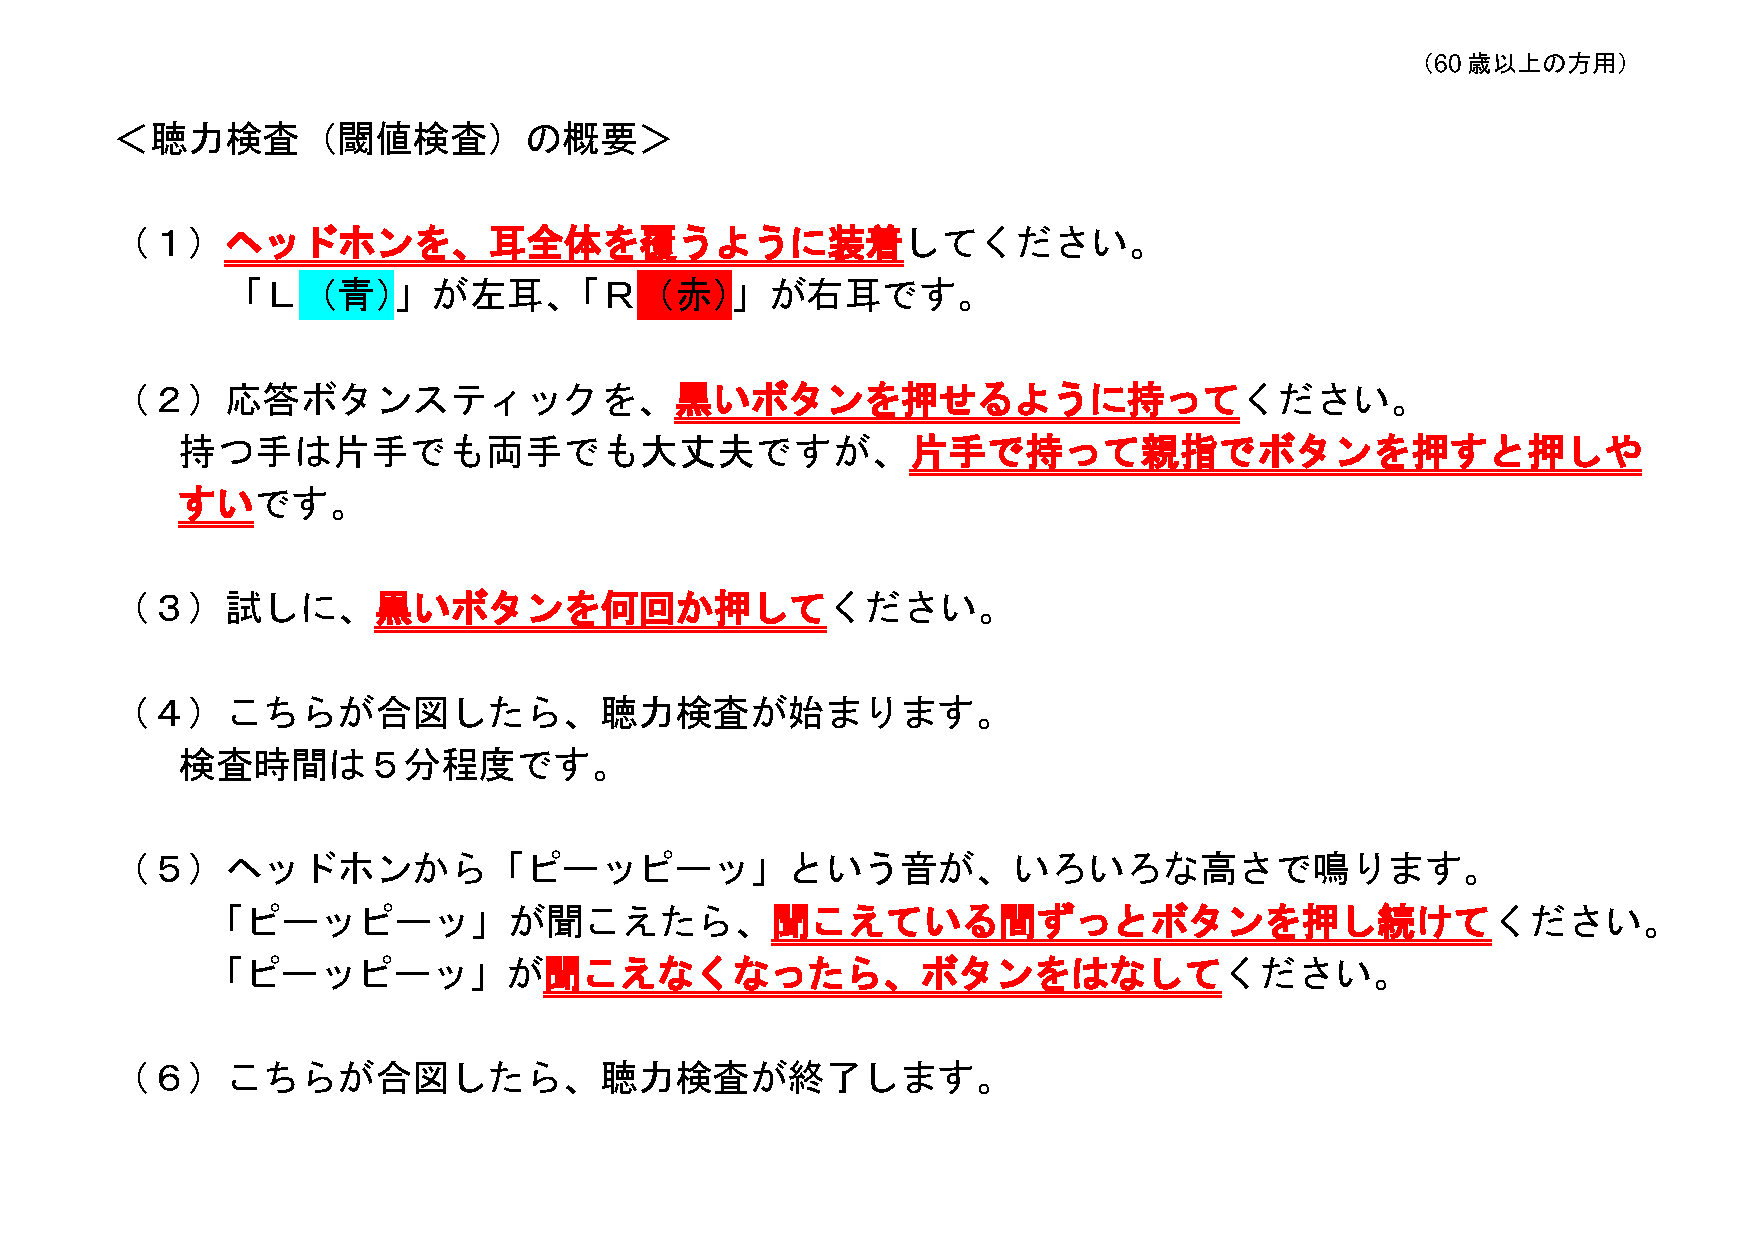
\includegraphics[scale=0.4]{furoku_A/MoreThan60_tyouryoku.pdf}
  \caption{聴力検査手順説明ボード}
\end{figure}
\begin{figure}[ht]
  \centering
  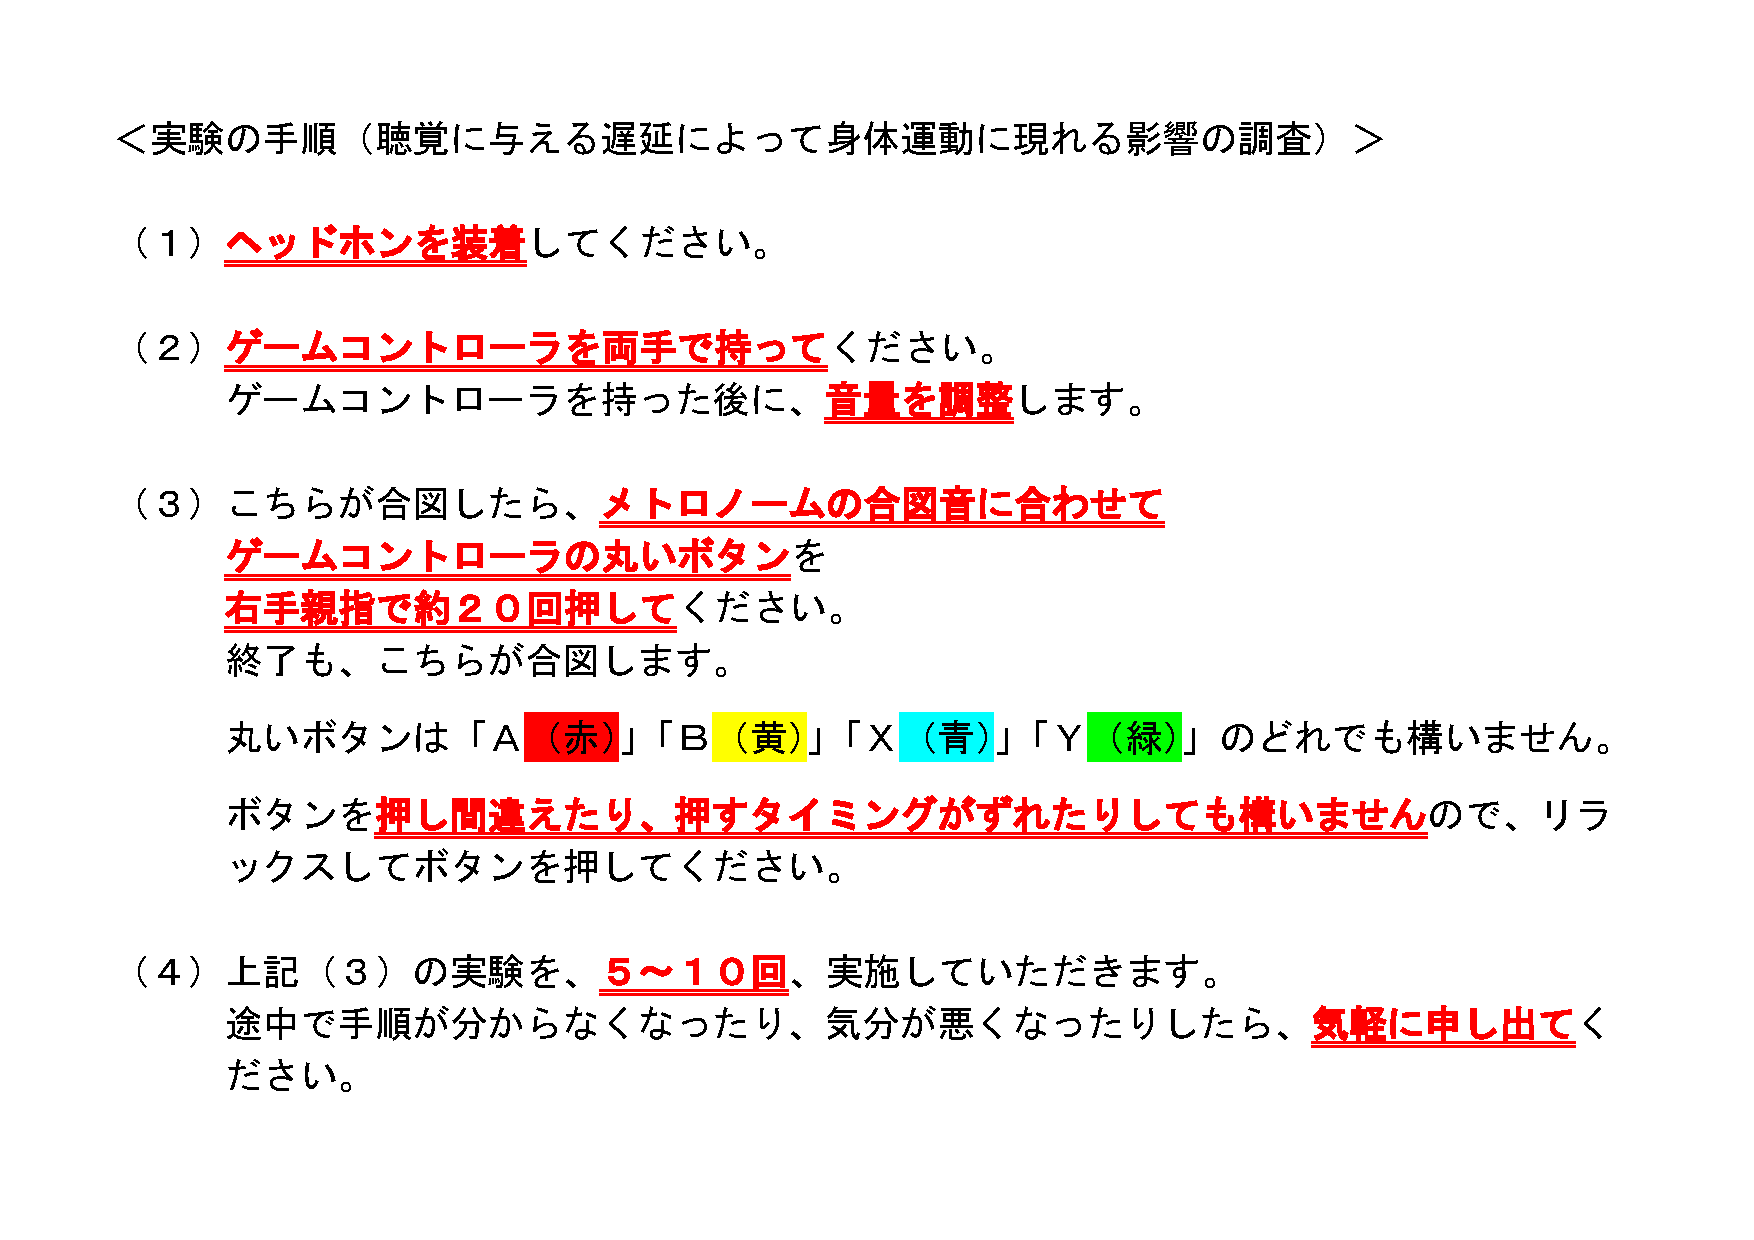
\includegraphics[scale=0.4]{furoku_A/Less60_Tezyunn.pdf}
  \caption{実験手順説明ボード(60歳未満の方用)}
\end{figure}
\begin{figure}[ht]
  \centering
  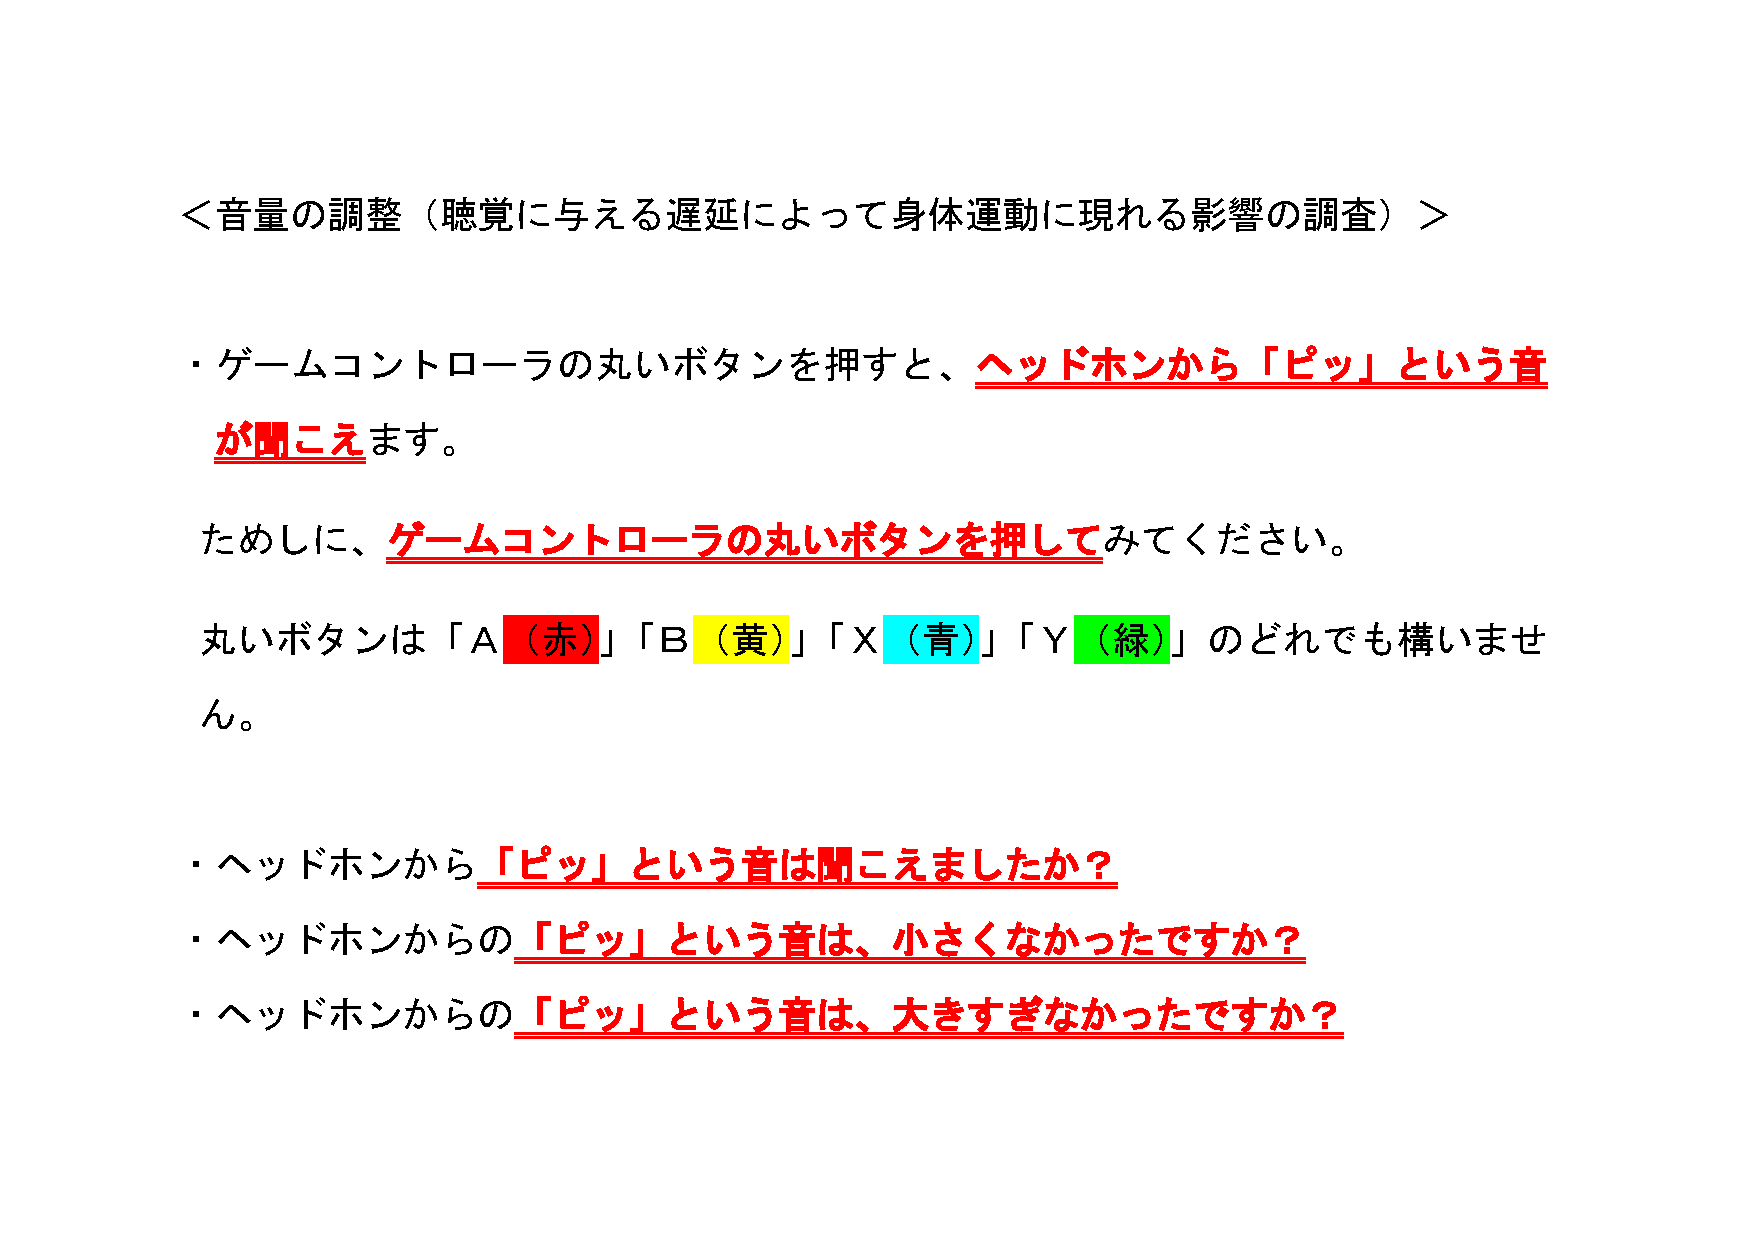
\includegraphics[scale=0.4]{furoku_A/Onnryou.pdf}
  \caption{音量調整ボード}
\end{figure}
